\chapter{\textit{Orthogonal Filter Bank Mutlicarrier} - OFDM} \label{capitulo2}

O OFDM é uma forma de onda bastante conhecida. Aqui, mais do que se apresentar a arquitetura utilizada para construção e detecção deste tipo de sinal, deseja-se mostrar como este tipo de símbolo continuará a ser utilizado em sistemas 5G e quais adaptações serão necessárias se houver alguma. Na próxima seção, introduz-se o leitor ao sistema. 

\section{Arquitetura OFDM}\label{pulso} 

\par O OFDM é uma tecnologia descoberta  há algumas décadas \ref{tcc1}, mas que somente entrou em uso recentemente, quando a tecnologia disponível em termos de software e circuitos eletrônicos, aliada às necessidades do mercado, possibilitaram sua aplicação prática.
\par Esta forma de onda é um caso especial do FDM (Frequency Division Multiplexing), uma técnica que data dos anos 1910 \cite{tcc1}, em que uma largura de banda larga é dividia entre vários usuários, sendo cada um deles alocados a uma faixa de frequências distinta. 
\par À época da telegrafia, fazia-se uso do TDM (“Time Divsion Multiplexing”), em que usuários eram alocados em slots de tempo de forma alternada. O sistema possuía algumas limitações, o que incentivava a busca por novas formas de alocar recursos do canal. Foi nesse contexto que surgiu a hipótese  da transmissão FDM \cite{tcc1}. 
\par Nomes como Alexander Graham Bell, Elisha Gray e Thomas Edison trabalharam no desenvolvimento desta tecnologia, tendo o primeiro se dedicado a aplicações desta na telefonia e não apenas na comunicação telegráfica.
\par O FDM tornou-se a base da telefonia analógica em 1918, sendo substituído por um sistema misto (TDM/FDM) nos anos 1970 e posteriormente por outro, unicamente TDM \cite{tcc1}.
\par Com o crescimento do número de usuários, o TDM tornou-se obsoleto e o FDM voltou a ser aplicado, mas em uma versão aprimorada. As informações passaram a ser transmitidas por canais mais estreitos, o que aumentou a imunidade destes a canais de multipercursos. Além disso, a equalização do sinal recebido tornou-se mais simples. 
\par Como qualquer sistema, o FDM também possui desvantagens. Para que não haja interferência entre canais adjacentes, é necessária a alocação de uma banda de guarda entre eles, um desperdício de recurso espectral. Outro problema é sua alta complexidade, já que são necessários moduladores ajustados à frequência de cada canal. 
\par Buscando solucionar estes inconvenientes, surge o conceito do OFDM, um sistema FDM com canais sobrepostos, mas não interferentes. Uma escolha simples que possibilita essas características são as portadoras regidas por funções senoidais harmônicas, que são ortogonais dentro do período fundamental. 		
Em um sistema OFDM, as $M$ subportadoras são representadas por $Re\{e^{j(2 \pi f_{m})}\}_{m = 0}^{M-1}$, $f_{m} = \frac{m+1}{T}$, em que $T$ é a duração do símbolo OFDM transmitido. Um bloco de sinal OFDM pode ser definido, então, como a soma de várias ondas senoidais de frequências distintas, pensando em cada uma como um subcanal. Na ausência de distorções, estes subcanais não se interferem, já que os pontos de máximo de uma subportadora coincidem com o de zero das outras. A Figura \ref{subportadorasOFDM}mostra este efeito da ortogonalidade em um sistema OFDM.

\begin{figure}[h!]
\centering
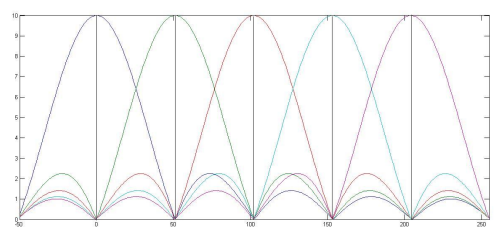
\includegraphics[width=3.5in]{fig_OFDM_freq.png} %Trocar para subortadoras OFDM
\caption{Subportadoras OFDM}
\label{subportadorasOFDM}
\end{figure}

\par A representação das subportadoras OFDM remete a uma função conhecida: a transformada inversa de Fourier – dada pela IDFT (Inverse Descrete Fourier Transform) no domínio discreto dos símbolos transmitidos, como será visto na seção \ref{trans_OFDM}  

\subsection{TRANSMISSOR OFDM}\label{trans_OFDM}
\par O transmissor OFDM é caracterizado da seguinte forma: primeiro, uma sequência de bits é mapeada em uma sequência de símbolos $X[k]$, M-PSK ou M-QAM. Esta sequência de símbolos em série é convertida em N fluxos de símbolos paralelos e cada um deles é transmitido por uma subportadora diferente $f_{m} =  \frac{m+1}{T}$, como mostra a Figura \ref{trans1OFDM} \cite{tcc9}.

\begin{figure}[h!]
\centering
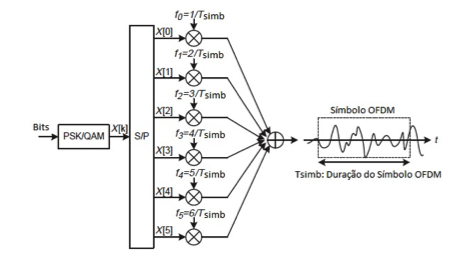
\includegraphics[width=3.5in]{trans_OFDM.png} %Trocar para subortadoras OFDM
\caption{Transmissior OFDM \cite{tcc9}}
\label{trans1OFDM}
\end{figure}

\par O símbolo OFDM transmitido pode ser escrito, no tempo discreto, como \cite{tcc9}

\begin{equation}\label{IDFTsimb}
x_{l}[n] = \sum_{k=0}^{M-1}X_{l}[k]e^{(j\frac{2\pi m n}{M})}, m=0,1,…,M-1,
\end{equation}

em que a equação \ref{IDFTsimb} representa a IDFT dos símbolos $X_{l}[k]_{k=0}^{M-1}$, que pode ser eficientemente computada por meio de do algoritmo de IFFT (Inverse Fourier Transform) \cite{tcc9}. Nesta equação, o subíndice l representa o l-ésimo símbolo transmitido na k-ésima suportadora.  O transmissor OFDM com o bloco IFFT é mostrado na Figura \ref{transIFFT}.

\begin{figure}[h!]
\centering
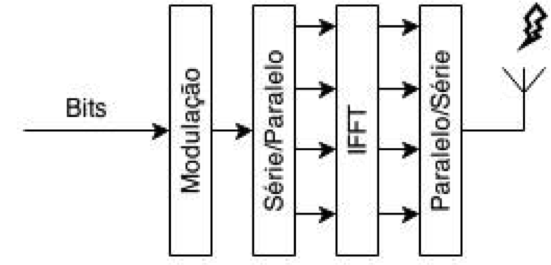
\includegraphics[width=3.5in]{transOFDMIFFT.png} %Trocar para sistema FDM
\caption{Transmissor OFDM com IFFT}
\label{transIFFT}
\end{figure}

\par O sistema OFDM da maneira que foi descrito acima só funcionaria na ausência de qualquer perturbação externa. Um efeito que traria grandes perturbações, seria a presença de um canal de multipercursos na transmissão, como será visto na Subseção \ref{multipercurso}. 

\subsection{Efeitos do Canal de Multipercursos}\label{multipercurso}

Seja o i-ésimo símbolo OFDM dado por \cite{tcc9}

\begin{equation}
x_{l}(t) = \sum_{m=0}^{M-1}X_{l}[m]e^{j 2 \pi f_{m}(t-lT)}
\end{equation}
	
\par Para um canal com resposta ao impulso $c_{l}(t)$, o sinal recebido será \cite{tcc9}:

\begin{equation}\label{eq3}
y_{l} (t)= x_{l}(t)\ast c_{l}(t)+ z_{l}(t)= \int_{0}^{\infty} c_{l}(t)x_{l}(t-\tau)dt+ z_{l}(t)
\end{equation}

em que, $z(t)$ representa ruído AWGN (Additve Gaussian White Noise – Ruído Branco Gaussiano Aditivo). No domínio discreto, a equação \ref{eq3} pode ser escrita como \cite{tcc9}:

\begin{equation} \label{eq4}
y_{l} = x_{l}[n] \ast c_{l}[n] + z_{l}[n] = \sum_{m=0}^{\infty}h_{l}[k]x_{l}[n-k]+z_{l}[n]
\end{equation}
	
\par Agora, se supõe que todo o segundo símbolo OFDM é enviado imediatamente após a última amostra do primeiro símbolo OFDM. Em acordo com a equação \ref{eq4}, o primeiro símbolo OFDM será prolongado no tempo, interferindo, portanto, nas amostras iniciais do segundo, como é mostrado pelo destaque em vermelho na Figura \ref{multichan}
	
\begin{figure}[h!]
\centering
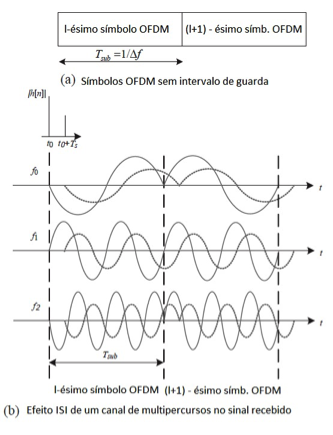
\includegraphics[width=3.5in]{ISIOFDM.png} %Trocar para sistema FDM
\caption{Interferência Intersimbólica \cite{tcc9}}
\label{multichan}
\end{figure}

\par É bastante intuitivo acrescentar um intervalo de guarda entre os símbolos OFDM. Este intervalo deve ser tal que sua duração supere o máximo atraso gerado pelo canal.  
\par Em vez de esperar um intervalo de tempo para o envio do próximo símbolo (zero-padding), é mais interessante construir o intervalo de guarda como mostra a Figura \ref{cp}

\begin{figure}[h!]
\centering
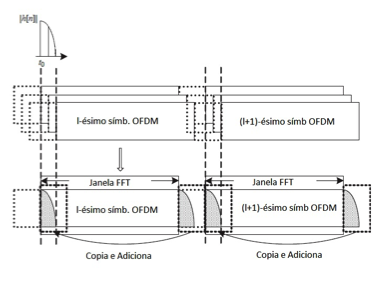
\includegraphics[width=3.5in]{cp.png} %Trocar para CP
\caption{Prefixo Cíclico  \cite{tcc9}}
\label{cp}
\end{figure}
		
\par A Figura \ref{cp} é a ilustração do processo conhecido por “inserção de prefixo cíclico”. A grande vantagem deste procedimento é a possibilidade de recuperação do sinal recebido por meio de da transformada de Fourier, como mostra o anexo I desta dissertãção. Na próxima seção apresenta-se o receptor OFDM. 

\subsection{Receptor OFDM}

\par No receptor, de forma geral, são desfeitos os passos do transmissor, como mostra a Figura \ref{rec_OFDM}.	

\begin{figure}[h!]
\centering
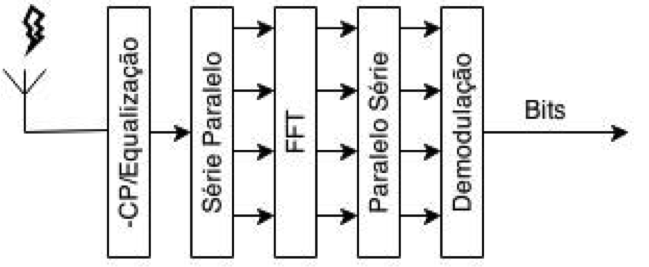
\includegraphics[width=3.5in]{recOFDM.png} %Trocar receptor OFDM
\caption{Receptor OFDM  \cite{tcc9}}
\label{rec_OFDM}
\end{figure}	

\par Primeiramente, o prefixo cíclico é eliminado. Após sua retirada, a equalização de um tap é realizada \ref{equalizationOFDM}:

\begin{equation}\label{equalizationOFDM}
x_{l}[n]=IFFT\{FFT\{(Y_{l}[m])/(H_{l}[m])\}\}
\end{equation}

\par Os símbolos $x_{l}[n]$ em série são convertidos em símbolos em paralelo e posteriormente demodulados, retornando às suas bandas-base por meio da FFT. O procedimento seguinte é a conversão paralelo-série, seguido pela demodulação. Finalmente, são obtidas estimativas dos bits enviados pelo transmissor. 

\begin{figure}[h!]
\centering
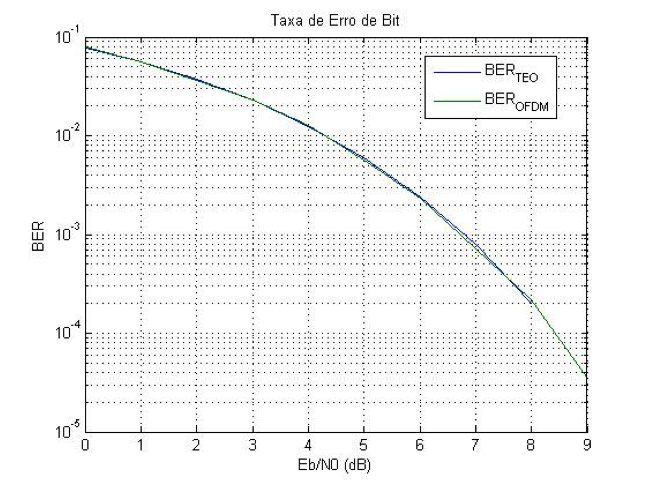
\includegraphics[width=3.5in]{BER_TEO.png} 
\caption{BER QPSK}
\label{taxa_erros}
\end{figure}

\par A taxa de erros desta estimativa na recepção é mostrada na Figura \ref{taxa_erros}. Esta figura foi obtida por meio de de simulação no software MATLAB© e os parâmetros utilizados são mostrados na tabela \ref{tab_sim}. 

\begin{center} \label{tab_sim}
\begin{tabular}{ c c}
Número de Subportadoras & 300  \\ 
Prefixo Cíclico & 32 \\  
Número de Símbolos & 50 \\
\end{tabular}
\end{center}

\par Percebe-se a partir da Figura 2.8, que o OFDM tem um desempenho próximo ao esperado para um sistema de portadoras únicas ($BER_{TEO}$). É válido ressaltar a queda de desempenho do sistema OFDM é causada pelo prefixo cíclico, que leva a um certo desperdício de energia.  
\par Até aqui, pode-se observar a existência de algumas vantagens no uso do OFDM:
\begin{itemize}	
    \item implementação Digital por meio da FFT/IFFT;
	\item eficiência espectral em comparação aos sistemas FDM comuns.
	\item taxa de erro de bits aceitável;
	\item equalização cuja complexidade independe do canal.
\end{itemize}   
\par Devido a estas vantagens, o sistema OFDM passou a ser aplicado em diferentes sistemas de comunicação. Alguns deles serão descritos na próxima seção, que abrange, também, as expectativas 5G para o OFDM.

\section{Aplicações OFDM - 4G x 5G}

\subsection{F-OFDM}
\subsection{ZT-DS-OFDM}



\section{Desempenho sob o efeito de não linearidades }
 



